\section*{Výsledky měření}
\subsection*{Kundtova trubice}
Rychlost zvuku ve vzduchu budeme používat hodnotu změřenou metodou uzavřeného rezonátoru při konstantní délce rezonátoru: $c_2 = \SI{345.7(3)}{\m\per\s}$~(viz níže).

Obrazec jako na obrázku \ref{obr::obrazectrubice} jsme pozorovali při délce trubice v rozmezí \num{60.0}--\SI{62.6}{\cm}.
Pozorovaný obrazec odpovídal přesně tomu na obrázku v tom smyslu, že délka trubice byla rovna čtyřem polovinám vlnové délky. 
Nejviditelnější byl obrazec právě při délce \SI{62.6}{\cm}, ale při délce \SI{62.8}{\cm} se již neobjevil vůbec.
Předpokládáme, že hodnoty byly rovnoměrně rozděleny v tomto intervalu, střední hodnotu určíme jako jeho střed a standardní odchylku vlnové délky počítáme po vydělení dvěma jako \mbox{$\sigma_{\lambda_2} = (\num{62.6}-\num{60.0})/(2\sqrt{12})~\si{\cm}$}.

Naměřená vlnová délka ve vzduchu tedy byla $\lambda_2 =~\SI{30.7(4)}{\cm}$.

Délka tyče byla $l_T = \SI{150.9(1)}{\cm}$.
Po dosazení do \eqref{eq::lambda1tyc} a vypočtení standardní odchylky $\sigma_{\lambda_1}=2 \lambda_1 \cdot \sigma_{l_T} / l_T$ dostáváme vlnovou délku v tyči $\lambda_1 =~\SI{301.8(2)}{\cm}$.

Dosazením do \eqref{eq::kundt_rovnost_frekvenci} dostáváme rychlost zvuku v tyči $c_1 =~\SI{3404(42)}{\m\per\s}$.
Standardní odchylku počítáme podle
\begin{equation}
\sigma _{c_1} = c_1 \cdot \sqrt{  \left( \frac{\sigma _{c_2}}{c_2}  \right)^2   +    \left( \frac{\sigma _{\lambda_1}}{\lambda_1}  \right)^2     +    \left( \frac{\sigma _{\lambda_2}}{\lambda_2}  \right)^2  } \,.
\end{equation}

Dosazením této hodnoty do \eqref{eq::modulpruznosti} vypočítáme modul pružnosti v tahu mosazi $E=~\SI{99(3)}{\GPa}$. 
Standardní odchylku počítáme podle
\begin{equation}
\sigma _E = E \cdot \sqrt{ \left( 2 \frac{\sigma _{c_1}}{c_1} \right)^2 +   \left( \frac{\sigma_\rho}{\rho}\right)^2} \,.
\end{equation}





\subsection*{Uzavřený rezonátor}
Při konstantní délce rezonátoru jsme našli základní frekvenci pro vzduch \SI{213}{\Hz} a pro oxid uhličitý \SI{162}{\Hz}.
Všechny naměřené rezonanční frekvence jsou uvedeny v tabulce \ref{tab::plynf} a zaneseny do grafu \ref{grp::graff}.
Frekvence, u nichž není uvedeno číslo $k$, nebyly celočíselnými násobky základní frekvence.
Pravděpodobně se jednalo o tzv. vlčí frekvence, tyto hodnoty jsme vyřadili ze zpracování.


\begin{tabulka}[htbp]
\centering
\begin{tabular}{cc|cc||cc|cc|cc}
\multicolumn{4}{c||}{vzduch} & \multicolumn{6}{c}{oxid uhličitý} \\
$k$ & $f~(\si{\Hz})$ & $k$ & $f~(\si{\Hz})$ & $k$ & $f~(\si{\Hz})$ & $k$ & $f~(\si{\Hz})$ & $k$ & $f~(\si{\Hz})$\\ \hline
1 & 213 & 8 & 1728 & 1 & 162 & 8 & 1347 & 16 & 2692 \\
--- & 324 & 9 & 1941 & 2 & 338 & 9 & 1511 & 17 & 2858 \\
2 & 436 & 10 & 2159 & --- & 486 & 10 & 1681 & 18 & 3028 \\
3 & 650 & 11 & 2375 & --- & 523 & 11 & 1851 & & \\
4 & 872 & 12 & 2597 & 4 & 675 & 12 & 2018 & & \\
5 & 1078 & 13 & 2806 & 5 & 838 & 13 & 2184 & & \\
6 & 1297 & 14 & 3023 & 6 & 1009 & 14 & 2354 & & \\
7 & 1515 & & & 7 & 1179 & 15 & 2524 & & \\
\end{tabular}
\caption{Naměřené rezonanční frekvence při délce rezonátoru $l=\SI{800}{\mm}$}
\label{tab::plynf}
\end{tabulka}

\begin{graph}[htbp] 
\centering
% GNUPLOT: LaTeX picture with Postscript
\begingroup
  \makeatletter
  \providecommand\color[2][]{%
    \GenericError{(gnuplot) \space\space\space\@spaces}{%
      Package color not loaded in conjunction with
      terminal option `colourtext'%
    }{See the gnuplot documentation for explanation.%
    }{Either use 'blacktext' in gnuplot or load the package
      color.sty in LaTeX.}%
    \renewcommand\color[2][]{}%
  }%
  \providecommand\includegraphics[2][]{%
    \GenericError{(gnuplot) \space\space\space\@spaces}{%
      Package graphicx or graphics not loaded%
    }{See the gnuplot documentation for explanation.%
    }{The gnuplot epslatex terminal needs graphicx.sty or graphics.sty.}%
    \renewcommand\includegraphics[2][]{}%
  }%
  \providecommand\rotatebox[2]{#2}%
  \@ifundefined{ifGPcolor}{%
    \newif\ifGPcolor
    \GPcolorfalse
  }{}%
  \@ifundefined{ifGPblacktext}{%
    \newif\ifGPblacktext
    \GPblacktexttrue
  }{}%
  % define a \g@addto@macro without @ in the name:
  \let\gplgaddtomacro\g@addto@macro
  % define empty templates for all commands taking text:
  \gdef\gplbacktext{}%
  \gdef\gplfronttext{}%
  \makeatother
  \ifGPblacktext
    % no textcolor at all
    \def\colorrgb#1{}%
    \def\colorgray#1{}%
  \else
    % gray or color?
    \ifGPcolor
      \def\colorrgb#1{\color[rgb]{#1}}%
      \def\colorgray#1{\color[gray]{#1}}%
      \expandafter\def\csname LTw\endcsname{\color{white}}%
      \expandafter\def\csname LTb\endcsname{\color{black}}%
      \expandafter\def\csname LTa\endcsname{\color{black}}%
      \expandafter\def\csname LT0\endcsname{\color[rgb]{1,0,0}}%
      \expandafter\def\csname LT1\endcsname{\color[rgb]{0,1,0}}%
      \expandafter\def\csname LT2\endcsname{\color[rgb]{0,0,1}}%
      \expandafter\def\csname LT3\endcsname{\color[rgb]{1,0,1}}%
      \expandafter\def\csname LT4\endcsname{\color[rgb]{0,1,1}}%
      \expandafter\def\csname LT5\endcsname{\color[rgb]{1,1,0}}%
      \expandafter\def\csname LT6\endcsname{\color[rgb]{0,0,0}}%
      \expandafter\def\csname LT7\endcsname{\color[rgb]{1,0.3,0}}%
      \expandafter\def\csname LT8\endcsname{\color[rgb]{0.5,0.5,0.5}}%
    \else
      % gray
      \def\colorrgb#1{\color{black}}%
      \def\colorgray#1{\color[gray]{#1}}%
      \expandafter\def\csname LTw\endcsname{\color{white}}%
      \expandafter\def\csname LTb\endcsname{\color{black}}%
      \expandafter\def\csname LTa\endcsname{\color{black}}%
      \expandafter\def\csname LT0\endcsname{\color{black}}%
      \expandafter\def\csname LT1\endcsname{\color{black}}%
      \expandafter\def\csname LT2\endcsname{\color{black}}%
      \expandafter\def\csname LT3\endcsname{\color{black}}%
      \expandafter\def\csname LT4\endcsname{\color{black}}%
      \expandafter\def\csname LT5\endcsname{\color{black}}%
      \expandafter\def\csname LT6\endcsname{\color{black}}%
      \expandafter\def\csname LT7\endcsname{\color{black}}%
      \expandafter\def\csname LT8\endcsname{\color{black}}%
    \fi
  \fi
  \setlength{\unitlength}{0.0500bp}%
  \begin{picture}(7936.00,5102.00)%
    \gplgaddtomacro\gplbacktext{%
      \csname LTb\endcsname%
      \put(1078,704){\makebox(0,0)[r]{\strut{} 0}}%
      \csname LTb\endcsname%
      \put(1078,1294){\makebox(0,0)[r]{\strut{} 500}}%
      \csname LTb\endcsname%
      \put(1078,1885){\makebox(0,0)[r]{\strut{} 1000}}%
      \csname LTb\endcsname%
      \put(1078,2475){\makebox(0,0)[r]{\strut{} 1500}}%
      \csname LTb\endcsname%
      \put(1078,3066){\makebox(0,0)[r]{\strut{} 2000}}%
      \csname LTb\endcsname%
      \put(1078,3656){\makebox(0,0)[r]{\strut{} 2500}}%
      \csname LTb\endcsname%
      \put(1078,4247){\makebox(0,0)[r]{\strut{} 3000}}%
      \csname LTb\endcsname%
      \put(1078,4837){\makebox(0,0)[r]{\strut{} 3500}}%
      \csname LTb\endcsname%
      \put(1210,484){\makebox(0,0){\strut{} 0}}%
      \csname LTb\endcsname%
      \put(2792,484){\makebox(0,0){\strut{} 5}}%
      \csname LTb\endcsname%
      \put(4375,484){\makebox(0,0){\strut{} 10}}%
      \csname LTb\endcsname%
      \put(5957,484){\makebox(0,0){\strut{} 15}}%
      \csname LTb\endcsname%
      \put(7539,484){\makebox(0,0){\strut{} 20}}%
      \put(176,2770){\rotatebox{-270}{\makebox(0,0){\strut{}$f (\si{\Hz})$}}}%
      \put(4374,154){\makebox(0,0){\strut{}$k$}}%
      \csname LT0\endcsname%
      \put(3742,3184){\rotatebox{37}{\makebox(0,0)[l]{\strut{}vzduch}}}%
      \csname LT1\endcsname%
      \put(4849,2534){\rotatebox{28}{\makebox(0,0)[l]{\strut{}oxid uhličitý}}}%
    }%
    \gplgaddtomacro\gplfronttext{%
    }%
    \gplbacktext
    \put(0,0){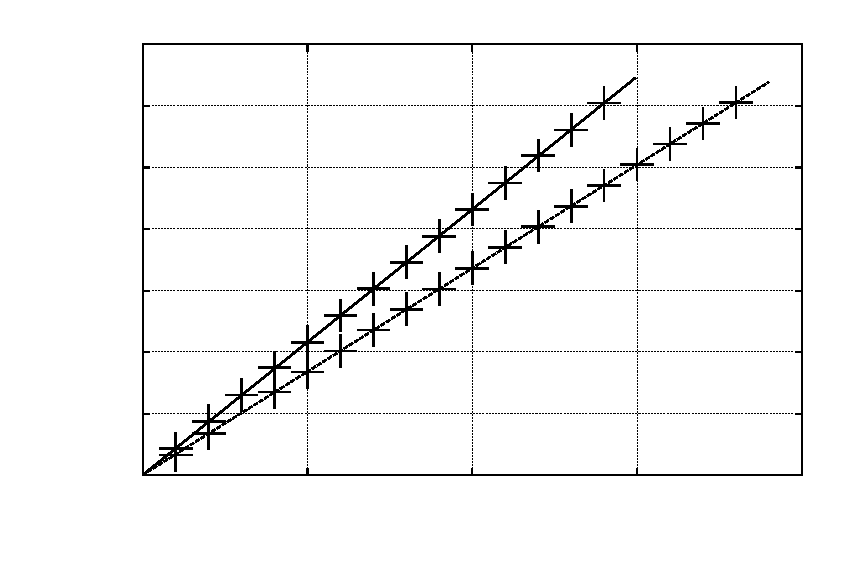
\includegraphics{graffrekvence}}%
    \gplfronttext
  \end{picture}%
\endgroup

\caption{Naměřená závislost rezonanční frekvence $f$ na čísle $k$ (viz rovnice \eqref{eq::f_na_k}) při délce rezonátoru \SI{800}{\mm}}
\label{grp::graff}
\end{graph}

\begin{graph}[htbp] 
\centering
% GNUPLOT: LaTeX picture with Postscript
\begingroup
  \makeatletter
  \providecommand\color[2][]{%
    \GenericError{(gnuplot) \space\space\space\@spaces}{%
      Package color not loaded in conjunction with
      terminal option `colourtext'%
    }{See the gnuplot documentation for explanation.%
    }{Either use 'blacktext' in gnuplot or load the package
      color.sty in LaTeX.}%
    \renewcommand\color[2][]{}%
  }%
  \providecommand\includegraphics[2][]{%
    \GenericError{(gnuplot) \space\space\space\@spaces}{%
      Package graphicx or graphics not loaded%
    }{See the gnuplot documentation for explanation.%
    }{The gnuplot epslatex terminal needs graphicx.sty or graphics.sty.}%
    \renewcommand\includegraphics[2][]{}%
  }%
  \providecommand\rotatebox[2]{#2}%
  \@ifundefined{ifGPcolor}{%
    \newif\ifGPcolor
    \GPcolorfalse
  }{}%
  \@ifundefined{ifGPblacktext}{%
    \newif\ifGPblacktext
    \GPblacktexttrue
  }{}%
  % define a \g@addto@macro without @ in the name:
  \let\gplgaddtomacro\g@addto@macro
  % define empty templates for all commands taking text:
  \gdef\gplbacktext{}%
  \gdef\gplfronttext{}%
  \makeatother
  \ifGPblacktext
    % no textcolor at all
    \def\colorrgb#1{}%
    \def\colorgray#1{}%
  \else
    % gray or color?
    \ifGPcolor
      \def\colorrgb#1{\color[rgb]{#1}}%
      \def\colorgray#1{\color[gray]{#1}}%
      \expandafter\def\csname LTw\endcsname{\color{white}}%
      \expandafter\def\csname LTb\endcsname{\color{black}}%
      \expandafter\def\csname LTa\endcsname{\color{black}}%
      \expandafter\def\csname LT0\endcsname{\color[rgb]{1,0,0}}%
      \expandafter\def\csname LT1\endcsname{\color[rgb]{0,1,0}}%
      \expandafter\def\csname LT2\endcsname{\color[rgb]{0,0,1}}%
      \expandafter\def\csname LT3\endcsname{\color[rgb]{1,0,1}}%
      \expandafter\def\csname LT4\endcsname{\color[rgb]{0,1,1}}%
      \expandafter\def\csname LT5\endcsname{\color[rgb]{1,1,0}}%
      \expandafter\def\csname LT6\endcsname{\color[rgb]{0,0,0}}%
      \expandafter\def\csname LT7\endcsname{\color[rgb]{1,0.3,0}}%
      \expandafter\def\csname LT8\endcsname{\color[rgb]{0.5,0.5,0.5}}%
    \else
      % gray
      \def\colorrgb#1{\color{black}}%
      \def\colorgray#1{\color[gray]{#1}}%
      \expandafter\def\csname LTw\endcsname{\color{white}}%
      \expandafter\def\csname LTb\endcsname{\color{black}}%
      \expandafter\def\csname LTa\endcsname{\color{black}}%
      \expandafter\def\csname LT0\endcsname{\color{black}}%
      \expandafter\def\csname LT1\endcsname{\color{black}}%
      \expandafter\def\csname LT2\endcsname{\color{black}}%
      \expandafter\def\csname LT3\endcsname{\color{black}}%
      \expandafter\def\csname LT4\endcsname{\color{black}}%
      \expandafter\def\csname LT5\endcsname{\color{black}}%
      \expandafter\def\csname LT6\endcsname{\color{black}}%
      \expandafter\def\csname LT7\endcsname{\color{black}}%
      \expandafter\def\csname LT8\endcsname{\color{black}}%
    \fi
  \fi
  \setlength{\unitlength}{0.0500bp}%
  \begin{picture}(5668.00,3968.00)%
    \gplgaddtomacro\gplbacktext{%
      \csname LTb\endcsname%
      \put(946,704){\makebox(0,0)[r]{\strut{} 700}}%
      \csname LTb\endcsname%
      \put(946,1454){\makebox(0,0)[r]{\strut{} 750}}%
      \csname LTb\endcsname%
      \put(946,2204){\makebox(0,0)[r]{\strut{} 800}}%
      \csname LTb\endcsname%
      \put(946,2953){\makebox(0,0)[r]{\strut{} 850}}%
      \csname LTb\endcsname%
      \put(946,3703){\makebox(0,0)[r]{\strut{} 900}}%
      \csname LTb\endcsname%
      \put(1977,484){\makebox(0,0){\strut{} 13}}%
      \csname LTb\endcsname%
      \put(3175,484){\makebox(0,0){\strut{} 14}}%
      \csname LTb\endcsname%
      \put(4373,484){\makebox(0,0){\strut{} 15}}%
      \put(176,2203){\rotatebox{-270}{\makebox(0,0){\strut{}$l(\si{\mm})$}}}%
      \put(3174,154){\makebox(0,0){\strut{}$k$}}%
    }%
    \gplgaddtomacro\gplfronttext{%
    }%
    \gplbacktext
    \put(0,0){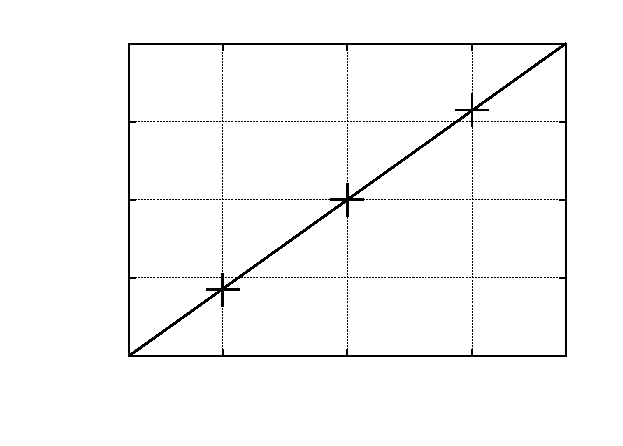
\includegraphics{grafdelka}}%
    \gplfronttext
  \end{picture}%
\endgroup

\caption{Délky rezonátoru, při kterých nastala rezonance (vzduch, $f=\SI{3025}{\Hz})$ }
\label{grp::grafl}
\end{graph}

Při konstantní frekvenci \SI{3025}{\Hz} jsme v rezonátoru naplněném vzduchem zaznamenali rezonanci při délkách rezonátoru uvedených v tabulce \ref{tab::vzduchl} a vynesených do grafu \ref{grp::grafl}.

\begin{tabulka}[htbp]
\centering
\begin{tabular}{cc}
$k$ & $l~(\si{mm})$ \\ \hline
13 & \num{742.5} \\
14 & \num{800.0} \\
15 & \num{857.5} \\
\end{tabular}
\caption{Délky rezonátoru, při kterých nastala rezonance (vzduch, $f=\SI{3025}{\Hz})$ }
\label{tab::vzduchl}
\end{tabulka}

Nafitované koeficienty $a$, $b$ a z nich pomocí \eqref{eq::cza} a \eqref{eq::czb} vypočtené rychlosti zvuku jsou uvedeny v tabulce \ref{tab::fit}. Odchylku rychlosti zvuku počítáme podle
\begin{equation}
\sigma_c = c \sqrt{ \left( \frac{\sigma_a}{a}   \right)^2
+ \left( \frac{\sigma_l}{l}   \right)^2 } 
\qquad \text{resp.} \qquad 
\sigma_c = c \sqrt{ \left( \frac{\sigma_b}{b}   \right)^2
+ \left( \frac{\sigma_f}{f}   \right)^2 }
\end{equation}


\begin{tabulka}[htbp]
\centering
\begin{tabular}{ccc}
\multirow{2}{*}{vzduch} & $a=~\SI{216.03(13)}{\Hz}$ & $\implies c=~\SI{345.7(3)}{\m\per\s}$ \\
& $b=~\SI{57.14(3)}{\mm}$ & $\implies c=~\SI{345.7(4)}{\m\per\s}$ \\ \hline
oxid uhličitý & $a=~\SI{168.17(10)}{\Hz}$ & $\implies c=~\SI{269.1(2)}{\m\per\s}$ \\
\end{tabular}
\caption{Nafitované koeficienty a vypočtené rychlosti zvuku pro metodu uzavřeného rezonátoru}
\label{tab::fit}
\end{tabulka}

Z naměřené rychlosti zvuku v oxidu uhličitém můžeme vypočítat jeho Poissonovu konstantu $\kappa$ podle \eqref{eq::kappa}.
Molekulová hmotnost oxidu uhličitého je $\mu=\SI{0.044}{\kg\per\mole}$.
Standardní odchylku počítáme jako
\begin{equation}
\sigma_\kappa = \kappa \cdot \sqrt{ \left(2\frac{\sigma_c}{c}\right)^2    +    \left( \frac{\sigma_T}{T} \right)^2} \,.
\end{equation}

Výsledná změřená Poissonova konstanta oxidu uhličitého je $\kappa =~\num{1.280(3)}$.